\section{5G SBA} \label{sota:sba}


The \ac{3GPP} specification for the \ac{5G} system architecture is defined to support data connectivity and services across a wide range of heterogeneous applications with diverse requirements. The 5G System adopts a \ac{SBA} with a modular and stateless \ac{NF} design, which segregates \ac{UP} and \ac{CP} functions for independent scalability and evolution. This architecture facilitates flexible deployment, where authorized \acp{NF} can access each other's services through reusable service procedures. The \ac{3GPP} TS \text{23.501} specification also identifies, among other key aspects, support for a unified authentication framework, discussed in Section \ref{sota:initiatives:CAPIF}, as well as analytics and capability exposure functionality, for third-party access, the latter of which will be analyzed in this section~\cite{ETSI_TS_123_501_V16_9_0}.

Figure \ref{fig:5g-sba} depicts the service-based representation of version \text{18.11.0} Release 18 of the Non-Roaming 5G System Architecture~\cite{ETSI_TS_123_501_V16_9_0}. It includes service-based interfaces (e.g. Nnef) for network function interaction within the \acl{CP}, as well as point-to-point reference points (e.g. N1) for interactions with \acl{UP} functions and entities (i.e \ac{UE}, (R)AN, \ac{UPF} and \ac{DN}).

\begin{figure}[htbp]
    \centering
    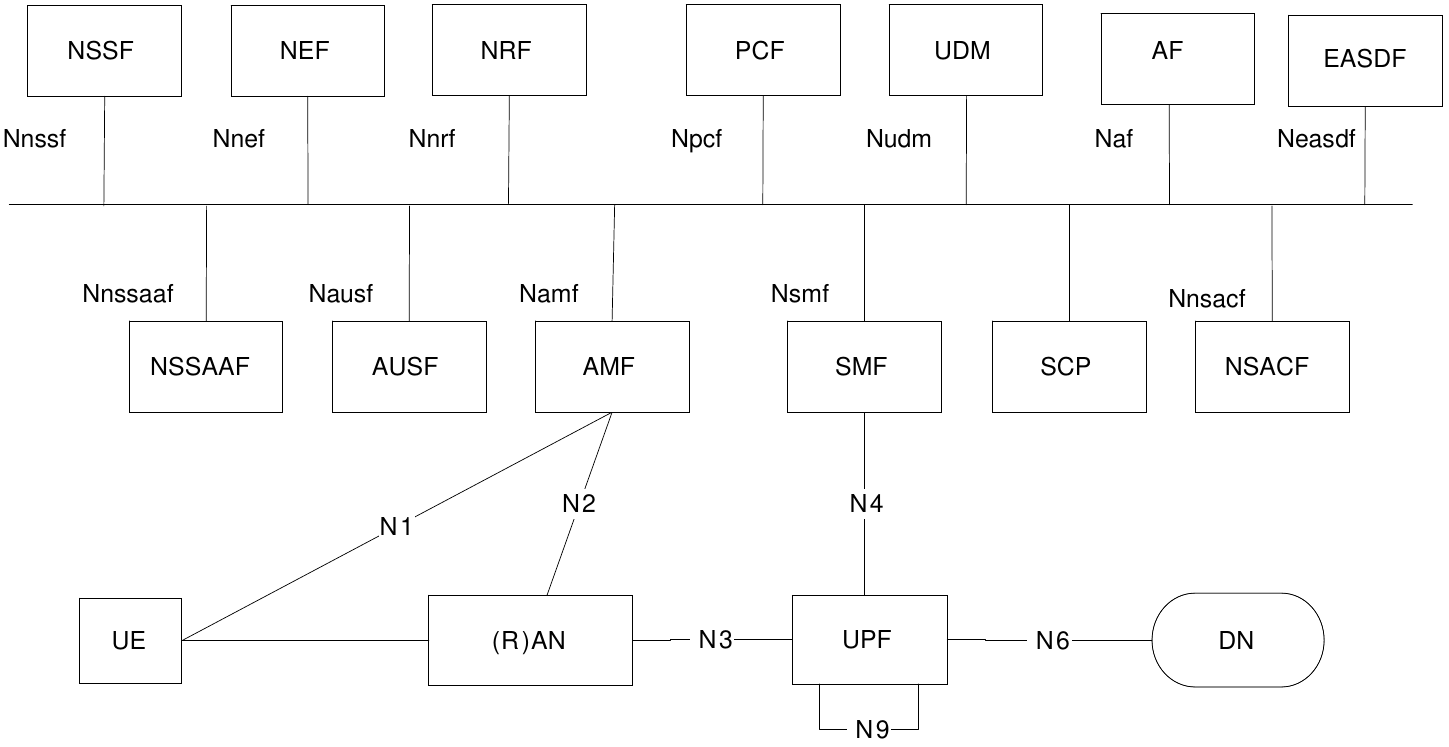
\includegraphics[width=1\linewidth]{figs/5G-SBA.png}
    \caption{Non-Roaming 5G System Architecture~\cite{ETSI_TS_123_501_V16_9_0}}
    \label{fig:5g-sba}
\end{figure}

\clearpage

The 5G System architecture consists of the following network functions:

\begin{itemize}
    \item{\textbf{(Radio) Access Network ((R)AN):}} access network that provides \ac{UE} connectivity to the \ac{5GC} Network, including NG-RAN and/or non-3GPP access technologies;

    \item{\textbf{\acf{DN}:}} external data network that provides access to operator services, third-party services or the Internet;

    \item{\textbf{\acf{AUSF}:}} supports authentication for both, 3GPP access and non-3GPP access (untrusted access via \acs{N3IWF}, trusted access via \acs{TNGF} and wireline access via \acs{W-AGF}). Its most significant functionalities include providing, to requester \acs{NF}, \acs{UE} authentication and protection mechanisms for \ac{SoR} information and \acs{UE} parameter updates;

    \item{\textbf{\acf{SMF}:}} handles \ac{PDU} session management (establishment, modification and release) and \ac{UE} \ac{IP} address allocation, including selecting and controlling the \ac{UPF} to steer traffic to the proper destination; 
    
    \item{\textbf{\acf{AMF}:}} responsible for registration, connection, reachability and mobility (e.g. handover) management between the \ac{UE} and the network. It also acts as an intermediary transport forwarding \ac{SM} messages between \acp{UE} and the \ac{SMF};

    \item{\textbf{\acf{PCF}:}} governs network behaviour based on a unified policy framework by providing policy rules to control plane functions that enforce them throughout the network. These policies cover, for example, charging, \acs{QoS} and network slicing scenarios (e.g. limits data rate per network slice). To facilitate these decisions, the \acs{PCF} accesses relevant subscription information from the \acs{UDR}, both located in the same \acs{PLMN}\hide{\later{explain this somewhere and PLMN too}};

    \item{\textbf{\acf{NSSAAF}:}} responsible for authentication and authorization mechanisms specific to a slice;

    \item{\textbf{\acf{NEF}:}} provides secure exposure of \acs{NF} capabilities and events to third parties, \acsp{AF} and edge computing environments, allowing them to interact with the network through standardized interfaces. It manages the secure provisioning of information from external applications to the internal network (e.g. authentication, authorization and assist in throttling \acsp{AF}), handling the necessary translation of data between the two domains (e.g. masking of network and user sensitive information to external \acsp{AF}'s according to the network policy). By interacting with other \acsp{NF}, namely the \acs{NWDAF}, NEF supports the exposure of \acs{NWDAF} analytics to external parties, mediating the collection of data by the \acs{NWDAF} and forwarding requests and notifications between it and the \acs{AF};

    \item{\textbf{\acf{UDM}:}} handles subscription management and access authorization based on subscription data (e.g. roaming restrictions). It is also responsible for registering and storing the \acp{NF} actively serving \acp{UE} (e.g. \ac{SMF} registration with the \ac{UDM} upon establishment of a \ac{PDU} session), which is specially relevant for service continuity (e.g. tracking \ac{SMF}-\ac{DNN} assignments of ongoing sessions);

    \item{\textbf{\acf{UPF}:}} provides an interconnection point through which external \ac{PDU} sessions connect to the \ac{DN}, handling packet routing and forwarding, such as uplink traffic between \acp{UE} and an instance of a \ac{DN}. It's also responsible for handling \ac{QoS} and policy rule enforcement within the user plane;

    \item{\textbf{\acf{AF}:}} interacts with the \ac{CN} to provide services, influencing aspects such as traffic routing, \ac{QoS} (e.g. request \acs{AF} session with required \ac{QoS}), policies and charging. Based on the deployment, \acsp{AF} considered to be trusted by the operator, as represented in Figure \ref{fig:5g-sba}, can interact directly with the rest of \acsp{NF}, whereas untrusted \acsp{AF} are required to access network function capabilities through the \acs{NEF};\hide{\later{maybe give examples}}

    \item{\textbf{\acf{SCP}:}} supports indirect communication between \acp{NF}' services, forwarding and routing messages either to the destination NF service or to a subsequent-hop \ac{SCP}. It also ensures communication security, as well as load balancing, monitoring, and overload control;

    \item{\textbf{\acf{NRF}:}} supports service decovery, allowing \acp{NF} to discover other \acp{NF} and their services, as well as SCP discovery by other SCPs. It achieves this by maintaining the current health status and profiles of available \ac{SCP} instances and \ac{NF} instances and their supported services. Additionally, it notifies subscribed consumers whenever a \ac{NF} or \ac{SCP} instance is registered, updated, or deregistered;

    \item{\textbf{\acf{NSSF}:}} responsible for selecting the Network Slice instances serving a specific \ac{UE}, tailored for specific service requirements. This includes determining the \ac{NSSAI} and, if needed, the mapping to the subscribed \acp{S-NSSAI};

    \item{\textbf{\acf{NWDAF}:}} collects and analyses data from the \ac{5G} network, leveraging information obtained from \acp{NF} (directly or via \ac{NEF}) and \ac{OAM} systems, with the goal of optimizing the 5G network's operation and service quality. \ac{NWDAF} consumers, i.e. \ac{5GC} \acp{NF} and \ac{OAM}, use the data analytics provided by the \ac{NWDAF} to assess, inter alia, slice's load level information, observed service experience, \ac{NF} load, network performance (e.g. \ac{gNB} status and resource usage) and \ac{QoS} Sustainability (e.g. \ac{QoS} change statistics). Analytics information are either statistical information on past events or predictive information (e.g. \ac{NF} load or network performance predictions, likelihood of a \ac{QoS} change) and can be obtained through the use of \ac{ML} models~\cite{ETSI_TS_123_288_V18_11_0}.

    

    % Lacks EASDF, NSACCF

\end{itemize}

\hide{

mention virtualization and softwarization

NFV and SDN

transition to a software-driven architec-
ture, emphasizing virtualization and cloud technologies, and
adopted a Service-Based Architecture (SBA) for scalable and
modular Network Functions (NFs)

scalable evolve indepedntly
}

\subsection{Network Analytics Capabilities}

The introduction of \ac{NWDAF} and its data collection, analytics and predictive capabilities, unlocks the possibility for data-driven network solutions that automate network management and optimize resource allocation~\cite{AdvancingPredictiveSecurity}. Capitalizing on this potential, several studies in the literature have explored various use cases for the \ac{NWDAF}, including solutions in network security and threat mitigation, as well as resource and operational efficiency. In the context of network security and threat mitigation, \ac{NWDAF} can, from collected data from functions such as the \ac{SMF}, \ac{AMF}, \ac{AF} and \ac{UPF}, identify abnormal user behavior and specific types of \ac{DDoS} attacks detecting UDP fragmentation, SYN, ICMP, DNS, and GTP flood attacks~\citep{AdvancingPredictiveSecurity,UserTerminalsAsAttackers}. This \ac{NWDAF} functionality can be extended to any anomaly detection scenarios in sectors such as logistics, maritime, and smart cities, where it can monitor communication patterns from vehicles, vessels or \ac{IoT} sensors to identify irregularities indicative of hijacking, system malfunctions or cyber-attacks~\cite{UserTerminalsAsAttackers}. Regarding resource and operational efficiency, the \ac{NWDAF} is capable of analysing \ac{RAN} data, \ac{UPF} traffic and CPU usage to predict network load and resource utilization, and proactively allocate additional resources when necessary, preventing performance degradation with faster response times than a simple threshold-based strategy~\cite{ExplorationNWDAFDevelopmentArchitecture6G}.


Additionally, the operation of the \ac{NWDAF} in conjunction with other \aclp{NF}, namely the \acs{NSSF}, supports automatic slice selection mechanisms with data collected and analysed by the \ac{NWDAF}. By evaluating \acs{QoS} and \acs{QoE} metrics and leveraging machine learning models, the network can dynamically select the most suitable vertical slices, acommodating a variety of \ac{IoT} use cases such as vehicular or real-time health systems~\cite{NetworkSliceSelectorIoT}.

\subsection{Network Exposure Capabilities} \label{sec:network:exposure:mechanisms}

The exposure of network capabilities has introduced a new level of flexibility for users and applications, allowing them to leverage and influence the capabilities of the network rather than being constrained by the functionalities explicitly offered by the mobile network. By granting access to third party external applications, this also opens the possiblility for telecom \acsp{SP} to monetize their network capabilities. With this objective, 3GPP has specified a series of Capability Exposure frameworks through the use of Northbound \acsp{API} and Application Enabler Layer \acsp{API}~\cite{CapabilityExposure3GPP}.

\subsubsection{\acl{NEF}} \label{sec:sba:nef}

The core network function responsible for \acs{5G}'s network capability exposure is the \acs{NEF}. The \acs{NEF} securely exposes \acsp{NF}' capabilities to external third parties, providing a set of northbound \acsp{API} through which they can interact with the \ac{5GC} to build network-aware applications. Thus, the \acs{NEF} allows service providers to access network capabilities contributing to the concept of an open and programmable network, while abstracting them from the underlying network~\cite{NEFsim}. More specifically, \acs{NEF} offers an exposure layer composed of northbound \acsp{API}, which are then internally connected to the \acs{SBA} southbound \acsp{API} to provide the intended functionalities, such as exposing network data and receiving management commands~\cite{CAPIFmicroserviceVerticals}. This and all other exposure capabilities supported by the \acs{NEF} can be classified into the following categories~\cite{ETSI_TS_123_501_V16_9_0}:
\begin{itemize}
    \item \textbf{Monitoring capability:}  monitoring of specific \acs{UE} events in the \acs{5G} System and making the correponding event information available for external exposure via the \acs{NEF}. Monitoring capability supports exposing \acs{UE}'s mobility management context such as \acs{UE} location, reachability, roaming status and loss of connectivity, as well as \acs{QoS} monitoring results. It includes functionality for identifying the \acs{5G} network function most suitable for configuring the specific monitoring events, detecting the monitoring event and reporting it to the authorised external party;
    
    \item \textbf{Provisioning capability:} allows an external party to provision information that can be used for the \acs{UE} in the \acs{5G} System. Provisioning Capability permits the external party to provision Expected \acs{UE} Behaviour, \acs{5G-VN} group information or service specific information to a \acs{5G} \acs{NF}. It comprises of the authorisation of the provisioning external third party, receiving the provisioned external information via the \acs{NEF} and storing and distributing it to the requiring \acsp{NF};
    
    \item \textbf{Policy/Charging capability:}  handling access and mobility management, \acs{QoS} and charging policies for the \acs{UE} based on a request from an external party. More specifically, it has mechanisms for handling a specific \acs{QoS}/priority setting for an \acs{UE} session and configuring the applicable charging party or charging rate;
    
    \item \textbf{Analytics reporting capability:} enables an external party to fetch, subscribe or unsubscribe to analytics information generated by the \acs{5G} System. Analytics reporting capability incorporates functionality for discovering the type of analytics available to an external party and requesting analytics information generated by the \acs{NWDAF} for consumption;

    \item \textbf{Member \acs{UE} selection capability:} allows an external party to acquire one or more list(s) of candidate \acs{UE}(s), selected from the list of target member \acs{UE}(s) provided by the \acs{AF}, along with additional information derived from assistance information generated by the \acs{5G} System based on predefined filtering criteria.

\end{itemize}


\subsubsection{Application Enabler Layer}

Unlike the previous generations, \acs{5G} focuses on enabling vertical applications integrated with the underlying \acs{5G} network, potentially providing \acsp{MNO} with new revenue streams and shifting away from traditional \acf{B2C} models, with an end-user, toward \acf{B2B} opportunities, with industry verticals~\cite{SEAL5GVerticals}. To capitalize on the monetization of their network capabilities while tailoring to the needs of the various vertical sectors, 3GPP has defined capability exposure frameworks based on Application Enabler Layer \acsp{API}. 

Application Enabler Layer \acsp{API} are abstraction layers for specific vertical applications (e.g. Edge, \acs{UAS}, {V2X}) or common to multiple vertical applications, which allow the exposure of common core and application enabler services to external applications. This abstraction is provided in paralell or on top of abstraction functionalities already provided by Network Northbound \acsp{API} via the \acs{NEF} or any other network \acsp{API} (e.g. network management \acsp{API}) to fullfill requests from vertical applications~\cite{CapabilityExposure3GPP}.

The Application Enabler Layer \acsp{API} designed to be common for multiple vertical applications are securely provided to verticals through the \acf{SEAL}~\cite{ETSI_TS_123_434_V18_12_0_SEAL}. The \acs{SEAL} defines a standardized functional architecture considering the common capabilities required to support multiple vertical applications over 3GPP networks. These capabilities are accessible for use through the following \acs{SEAL} services: Location management, Group management, Configuration management, Identity managemen, Key management, Network resource management, Data delivery, Notification management, Network slice capability enablement and Application data analytics enablement~\cite{ETSI_TS_123_434_V18_12_0_SEAL}. Many of these capabilities correspond to auxiliary services that address cross-cutting concerns, common across verticals. Developing them independently for each vertical would be redundant and require substantial time and effort. Instead, vertical application developers can focus exclusively on the core features and functionalities of the vertical application, while utilizing \acs{SEAL} for the auxiliary services, thus saving significant time and cost to market~\cite{SEAL5GVerticals}.

In addition to \acs{SEAL}'s common reusable services across multiple vertical sectors, a dedicated service framework is required to address the specific requirements of edge-based services and edge computing. Edge Computing is a network architecture concept that deploys cloud computing capabilities and service environments close to the \acsp{UE}, with the goal of achieving several benefits, such as lower latency, higher bandwidth, reduced backhaul traffic and possibly new innovative services not feasible or supported in regular cloud environments. With this goal, 3GPP specifies an application architecture for enabling Edge Applications on the \acf{EDN}. More specifically, it introduces the \acf{EEL} to facilitate communication between the \acfp{AC} running on an \acs{UE} and the \acf{EAS} deployed on the \acs{EDN}. Regarding network exposure capabilities, the \acs{EEL} exposes northbound \acsp{API} towards the \acsp{EEC} (running on an \acs{UE}), \acsp{EAS} (possibly third-party \acsp{EAS} outside the \acsp{ECSP} trust domain) and other internal functional entities. These services encompass native \acs{EEL} services, such as service provisioning, \acs{EAS} discovery and support for service continuity, as well as enhanced re-exposed services of the 3GPP \acs{CN}, such as \acs{UE} Location and \acs{QoS} sessions. While distinct in their application, both categories utilize the exposed network capabilities via \acs{NEF} northbound \acsp{API}, optionally via \acs{CAPIF}. Native services consume these network capabilities to support internal logic, such as retrieving a \acs{UE}'s location to filter discovery results, whereas re-exposed services are built directly on the \acs{NEF} capabilities to provide enhanced access to network functions~\cite{ETSI_TS_123_558_V18_11_0_EDGE}.

The previously mentioned enabler layers focus on generic application support for multiple vertical applications and edge applications, respectively. To address the diverse requirements of heterogeneous vertical use cases, additional vertical-specific enabler layers were defined. The \acf{VAE} layer ensures efficient use and deployment of \acs{V2X} applications on 3GPP networks, supporting use cases such as platooning, remote and tele-operated driving, \acs{HD} maps and Vehicle-to-Pedestrian communication with \acf{VRUP}. It serves as an abstraction layer that encapsulates the underlying mechanisms from the \acs{V2X} application specific layer and exposes them via northbound \acsp{API}, providing interfaces for operations such as group management and message distribution. To support these functionalities, the \acs{VAE} utilizes the \acs{NEF} for interacting with the \acs{5G} System, allowing it to receive \acs{QoS} monitoring information and network data analytics (e.g. congestion status reported by the \acs{NWDAF} to \acs{NEF}). It also relies on \acs{SEAL} for support services in location management, group management, configuration management, identity management, key management and network resource management, thus emphasizing the importance of these components in the \acs{V2X} vertical-specific scenario~\cite{ETSI_TS_123_286_V19_0_0_V2X}.

Similar enabler layers exist for other vertical sectors in \acf{UAS}~\cite{ETSI_TS_123_255_V18_2_0_UAS}, \acs{5G} messaging for \acf{MIoT} communication~\cite{ETSI_TS_123_554_V18_10_0_Messaging} and \acf{FF}~\cite{3GPP_23_745_V17_0_0_FF}. All provide abstraction layers for vertical specific capabilities, exposing northbound \acsp{API} that may require interactions with the \acs{NEF} and \acs{SEAL} components to fulfill these capabilities, optionally via \acs{CAPIF}.



\subsubsection{NEF Implementations} \label{exposure:NEFimplementations}

In regards to \ac{NEF} implementations, there are a variety of implementations across both open source 5G core solutions and in commercial deployments. This section provides an overview of the current \ac{5G} \ac{NEF} solutions and their supported northbound \acsp{API} and services, followed by a discussion of their level of adoption in the literature. 

Concerning commercial solutions, Nokia's \ac{NEF}~\cite{NokiaNEF2022} is described as a cloud native \ac{PaaS} following a microservices architecture with a \ac{REST} aproach. However, proprietary commercial solutions are constrained by licensing restrictions, making free and open-source alternatives more viable.

As for open source projects, the presence of the \ac{NEF} component varies across different \ac{5G} core implementations. For instance, Open5GS, despite providing a C-based implementation of a \ac{5G SA} Core with a \ac{SBA} architecture supporting a wide variety of network functions, it still lacks a \ac{NEF} implementation~\cite{Open5GSDocs}. Consequently, authors have resorted to extending the Open5GS \acs{CN} by developing and integrating their own \ac{NEF} solutions~\citep{CloudEnabledDeployment5GN, DynamicQoSAdaptationviaExposedServiceAPIs}. The \ac{5G} \ac{CN} provided by the \ac{OAI} software alliance does not provide \ac{NEF} functionality either, with support expected in a future release scheduled for the first semester of 2026~\cite{OpenAirInterface5GCN}. In constrast, Free5GC, by the Linux Foundation, includes a partial \ac{NEF} implementation~\cite{Free5GC-NEF}, enabling exposure of network capabilities through services such as \texttt{Nnef\_PFDManagement} and \texttt{Nnef\_TrafficInfluence}, as defined in 3GPP TS 23.502~\cite{3GPP-23.502}. However, certain inconsistencies exist, notably regarding traffic steering capabilities via the \ac{NEF}, which are available in version 3.4.5 but absent in version 4.0.0~\cite{Free5GCv4.0.0NotSupportTrafficSteering}.

% Nnef\_PFDManagement       -> PfdManagementAPI     (TS 29.122)
% NNef\_TrafficInfluence    -> TrafficInfluenceAPI  (TS 29.522)

However, to the author's best knowledge, the level of adoption to actual \ac{NEF} implementations remains relatively low in the research community, at least in the researched body of literature considered in this dissertation. Despite the first release of Free5GC's \ac{NEF} being introduced on 12 November 2024, subsequent research papers in 2025 still do not utilize this implementation~\cite{LoadBalancingConnectedVehicleServices}\hide{\later{only one paper for this, should be at least 2}}, instead extending the \acs{CN} with custom \ac{NEF} solutions.

An alternative approach to these implementations is the open-source \ac{NEF} simulator NEFSim~\cite{NEFsim}, developed under the European project EVOLVED-5G. The component offers the standardized set of NEF northbound \acsp{API}, allowing their validation in a configurable and simulated environment. This proves especially valuable for testing and validation purposes aiding Network App developers to integrate \ac{NEF} clients into their applications, without requiring access to a full-blown \ac{NEF} instance. Thus, as the \ac{NEF} constitutes the main gateway to the \ac{5G} System, proper interaction with the \ac{NEF} ensures that Network Applications can also correctly interact with the \acs{5G} System~\cite{AutomatedTestingOrchestrationFramework}. The current implementation, extended at \acs{ITAv}, supports the PfdManagement, MonitoringEvent, AsSessionWithQoS and TrafficInfluence \acsp{API}, as per the \acs{3GPP} TS 29.522 northbound \acs{API} specification~\cite{ETSI_TS_129_522_V18_11_0}. Therefore, the NefSim supports a broader set of \acs{NEF} northbound \acsp{API}, as summarized in Table \ref{tab:nef:comparision:short}. This corresponds to a condensed version, with the full comparison encompassing all \acs{NEF} northbound \acsp{API} being presented in Table \ref{tab:nef:comparision:long} of the Appendix \ref{chap:appendix-more}. Additionally, among the analysed open-source implementations it is the only one that features \acs{CAPIF} integration, significantly reducing integration effort on adoption. 

\begin{table}[ht]
\centering
\renewcommand{\arraystretch}{1.3} % Increase row height
\rowcolors{2}{gray!15}{white}     % Alternating row colors
% Implemented ?
% $\checkmark$      -> yes
% $\times$          -> no
% $\LEFTcircle$     -> partially
\begin{tabular}{p{6cm} c c c}
\toprule
\textbf{Northbound \acs{API}} & \textbf{Free5GC} & \textbf{NEFSim} \\
\midrule
% Implemented ?
% $\checkmark$      -> yes
% $\times$          -> no
% $\LEFTcircle$     -> partially
PfdManagement                & $\checkmark$         & $\checkmark$ \\
MonitoringEvent              & $\times$             & $\checkmark$ \\
AsSessionWithQoS             & $\times$             & $\checkmark$ \\
TrafficInfluence             & $\checkmark$         & $\checkmark$ \\
\bottomrule
\end{tabular}

\caption{Northbound API Coverage across open source NEF Implementations}
\label{tab:nef:comparision:short}
\end{table}




\hide {

\later{Observation in other paper (cloud-native NEF and CAPIF interplay) regarding NEFSim: Still, NEFSim does not allow interacting with a CN or southbound, or refer to CAPIF. -> I also don't understand which NEF they actually use}

GIRL
- openness by enabling new levels of programmability in the core and edge
domains, which allows third-party innovators, also known as vertical industries, to control and monitor the deployment process and performance of their services
- securely made through the NEF's APIs, hiding all the underlying network topology, to external third parties that may use them to build network aware applications
- northbound APIs

OTHERS
cloud-enabled deployment of 5G Core network with analytics features -> However, NEF is not included in the most popular open source implementations of the 5GCN (OPEN5GS doesn't have NEF implemented)

(load-balancing-in-connected-vehicle) UERANSIM [18] for simulating UE and gNB.

}
